\ylDisplay{Lääts} % Ülesande nimi
{Tundmatu autor} % Autor
{lahtine} % Voor
{2007} % Aasta
{G 9} % Ülesande nr.
{7} % Raskustase
{
% Teema: Geomeetriline-optika
\ifStatement
Teritamata pliiatsi telg ühtib koondava läätse peateljega. Mitu korda on pliiatsi kujutise pikkus tema enda pikkusest erinev, kui pliiatsi ühe otsa kujutise diameetri ja pliiatsi diameetri suhe on $k_1$ ning teise otsa jaoks on see suhe $k_2$? Pliiatsi mõlemad otsad asuvad läätsest fookuskaugusest suuremal kaugusel.
\fi


\ifHint
Suhteliselt kindel meetod on avaldada kõik ülesandes antud ja otsitavad muutujad võimalikult mugavate jooniselt leitavate suuruste kaudu ning loota, et saadud võrranditest on lihtne näha, kuidas lõppvastus avaldub $k_1$ ja $k_2$ kaudu. Häda korral tuleb lahendada kolmest võrrandist koosnev võrrandisüsteem ($k_1$, $k_2$ ning otsitava suhte jaoks). Silmas peab pidama, et jooniselt valitud muutujad peavad ülesande geomeetria üheselt ära defineerima. Selleks sobivad näiteks läätse fookuskaugus ning pliiatsi mõlema otsa kaugused läätsest.
\fi


\ifSolution
Olgu pliiatsi otste kaugused läätsest $d_1 = |BO|$ ja $d_2 = |DO|$ ning pliiatsi kujutise otste kaugused läätsest vastavalt $f_1 = |B'O|$ ja $f_2 = |D'O|$ (vt joonist).

\begin{center}
	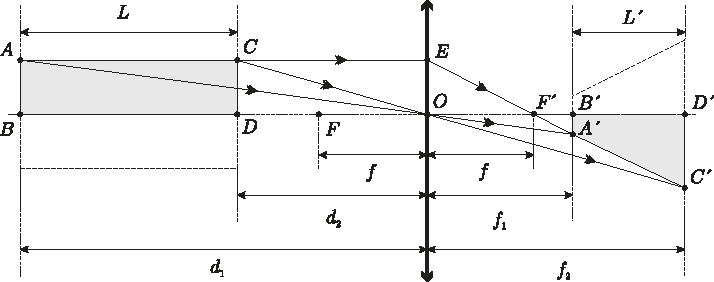
\includegraphics[width=\linewidth]{2007-lahg-09-lah}
\end{center}

Paneme kirja valemid suurendustegurite jaoks:
\[
k=\frac{L^{\prime}}{L}, \quad k_{1}=\frac{|A^{\prime}B^{\prime}|}{|AB|}, \quad k_{2}=\frac{|C^{\prime}D^{\prime}|}{|CD|}.
\]
Sarnastest kolmnurkadest $FB'A'$ ja $FOE$ leiame, et
\[
\frac{|A^{\prime}B^{\prime}|}{|EO|}=\frac{|F^{\prime}B^{\prime}|}{|FO|}=\frac{f_{1}-f}{f}.
\]
Analoogiliselt, sarnastest kolmnurkadest $FD'C'$ ja $FOE$ leiame, et
\[
\frac{|C^{\prime}D^{\prime}|}{|EO|}=\frac{|F^{\prime}D^{\prime}|}{|FO|}=\frac{f_{2}-f}{f}.
\]
Kuna $|EO| = |AB| = |CD|$, siis
\[
k=\frac{f_{2}-f_{1}}{d_{1}-d_{2}}, \quad k_{1}=\frac{f_{1}-f}{f}, \quad k_{2}=\frac{f_{2}-f}{f}.
\]
Kasutades läätse valemit mõlema otsa jaoks:
\[
\frac{1}{d_{1}}+\frac{1}{f_{1}}=\frac{1}{f} \quad \operatorname{ning} \quad \frac{1}{d_{2}}+\frac{1}{f_{2}}=\frac{1}{f}
\]
saame avaldada pikkused $d_1$ ja $d_2$ pikkuste $f_1$ ja $f_2$ kaudu:
\[
d_{1}=\frac{f_{1} f}{f_{1}-f}, \quad d_{2}=\frac{f_{2} f}{f_{2}-f}.
\]
Asendame saadud väärtused suurendusteguri $k$ avaldisse:
\[
\begin{aligned}
	k&=\frac{f_{2}-f_{1}}{f_{1}-f}-\frac{f_{2} f}{f_{2}-f}=\frac{f_{2}-f_{1}}{f} \frac{\left(f_{1}-f\right)\left(f_{2}-f\right)}{f_{1}\left(f_{2}-f\right)-f_{2}\left(f_{1}-f\right)} \\ 
	&=\frac{f_{2}-f_{1}}{f} \frac{\left(f_{1}-f\right)\left(f_{2}-f\right)}{f_{1} f_{2}-f_{1} f-f_{2} f_{1}+f_{2} f}=\frac{f_{2}-f_{1}}{f} \frac{\left(f_{1}-f\right)\left(f_{2}-f\right)}{f_{2} f-f_{1} f} \\ &=\frac{f_{2}-f_{1}}{f} \frac{\left(f_{1}-f\right)\left(f_{2}-f\right)}{f\left(f_{2}-f_{1}\right)}=\frac{\left(f_{1}-f\right)\left(f_{2}-f\right)}{f^{2}}.
\end{aligned}
\]
Võrreldes saadud avaldist varem saadud avaldistega $k_1$ ja $k_2$ jaoks, on lihtne näha, et
\[
k=\frac{f_{1}-f}{f} \frac{f_{2}-f}{f}=k_{1} k_{2}.
\]
\emph{Märkus}. Joonisel me mugavuse kaalutlusel tegelikult vaatleme vaid pool pliiatsit, aga on ilmne, et lahenduskäik kehtib ka terve pliiatsi kohta (joonisel on pliiatsi teine pool näidatud punktiirjoonega).
\fi
}